\documentclass[english]{sig-alternate}
\usepackage{color}
\usepackage{xcolor}
\usepackage{colortbl}
\usepackage{amstext}
\usepackage{pdfpages}
\usepackage{alltt}
\usepackage{epstopdf}
\usepackage{listings}
\lstset{basicstyle=\ttfamily,breaklines=true}
\usepackage{xspace,colortbl}
\usepackage[USenglish]{babel}
\usepackage{multirow}
\usepackage{url}
\usepackage{subfigure}
\usepackage{graphicx}
\usepackage{amssymb}
\usepackage{fmtcount}
\usepackage{amsfonts}
\usepackage{xspace}
\usepackage{amsmath}
\usepackage{multirow}
\usepackage[mathscr]{eucal}
\usepackage{times}
\usepackage{colortbl}
\usepackage{bm}
\usepackage[nospace]{cite}
\makeatletter
\newif\if@restonecol
\makeatother
\let\algorithm\relax
\let\endalgorithm\relax
\usepackage[lined,boxed,vlined,ruled]{algorithm2e}
\special{papersize=8.5in,11in}



\setcounter{secnumdepth}{3}

\long\def\comment#1{}
%\usepackage[dvipdfm]{hyperref}
%\usepackage[dvips]{hyperref}
\begin{document}
%\conferenceinfo{SIGMOD'14,} {June 22--27, 2014, Snowbird, Utah, USA.}
%\CopyrightYear{2014}
%\clubpenalty=10000
%\widowpenalty = 10000

%\hyphenpenalty=5000
\tolerance=1000
\linespread{1}%
%\pagenumbering{arabic}

\title{Wisteria: Nurturing Scalable Data Cleaning Infrastructure} 


\author{\large Daniel Haas,~~Sanjay Krishnan,~~Jiannan Wang,~~Michael J. Franklin,~~Eugene Wu{$\,^\dag$}\thanks{Work conducted while visiting UC Berkeley} \\
\vspace{.2em}\affaddr{\large UC Berkeley ~~~~ $^\dag$Columbia University} \\
\fontsize{9}{10}\selectfont\ttfamily\upshape
\vspace{.1em}\{dhaas,sanjay,jnwang,franklin\}@cs.berkeley.edu, ewu@cs.columbia.edu
}

\newcommand{\squishlist}{
   \begin{list}{$\bullet$}
    { \setlength{\itemsep}{0pt}
      \setlength{\parsep}{2pt}
      \setlength{\topsep}{6pt}
      \setlength{\partopsep}{0pt}
      \leftmargin=5pt
\rightmargin=0pt
\labelsep=5pt
\labelwidth=10pt
\itemindent=0pt
\listparindent=0pt
\itemsep=\parsep
    }
}
\newcommand{\squishend}{\end{list}}

%\linespread{0.96}


%Identifying Similarity Functions from Examples for Effective Record Matching

%\subtitle{[Extended Abstract]
%\titlenote{A full version of this p aper is available as
%\textit{Author's Guide to Preparing ACM SIG Proceedings Using
%\LaTeX$2_\epsilon$\ and BibTeX} at
%\texttt{www.acm.org/eaddress.htm}}}
%\pagenumbering{arabic}

\newtheorem{theorem}{Theorem}
\newtheorem{example}{Example}
\newtheorem{definition}{Definition}
\newtheorem{proposition}{Proposition}
\newtheorem{lemma}{Lemma}
\newtheorem{corollary}{Corollary}
\newtheorem{demonstration}{Demonstration}

\newcommand{\dataset}{data set\xspace}
\newcommand{\datasets}{data sets\xspace}
\newcommand{\biascorrected}{NormalizedSC\xspace}
\newcommand{\bias}{\biascorrected}
%\newcommand{\sampledirty}{\texttt{SampleDirty}\xspace}
%\newcommand{\sampleclean}{\texttt{SampleClean}\xspace}
%\newcommand{\allclean}{\texttt{AllClean}\xspace}
%\newcommand{\alldirty}{\texttt{AllDirty}\xspace}
\newcommand{\sampledirty}{{SampleDirty}\xspace}
\newcommand{\sampleclean}{{RawSC}\xspace}
\newcommand{\allclean}{{AllClean}\xspace}
\newcommand{\alldirty}{{AllDirty}\xspace}
\newcommand{\sys}{\textsf{Wisteria}\xspace}
\newcommand{\projx}{\sys}
\newcommand{\saqp}{SAQP\xspace}
\newcommand{\saqpplus}{\projx}
\newcommand{\blinkdb}{BlinkDB\xspace}
\newcommand{\ctable}{\ensuremath{T^{clean}}\xspace}
\newcommand{\var}{\ensuremath{\texttt{var}}\xspace}

\newcommand{\attr}[1]{\texttt{#1}\xspace}
\newcommand{\afunc}[1]{\texttt{#1}\xspace}
\newcommand{\M}{\ensuremath{M}\xspace}
\newcommand{\Pset}{\ensuremath{P}\xspace}
\newcommand{\gfunc}{\ensuremath{f}\xspace}
\newcommand{\avgfunc}{\ensuremath{\texttt{avg} }\xspace}
\newcommand{\varfunc}{\ensuremath{\texttt{var} }\xspace}
\newcommand{\productfunc}{\ensuremath{\texttt{product} }\xspace}
\newcommand{\geomeanfunc}{\ensuremath{\texttt{geomean} }\xspace}
\newcommand{\countfunc}{\ensuremath{\texttt{count} }\xspace}
\newcommand{\sumfunc}{\ensuremath{\texttt{sum} }\xspace}
\newcommand{\groupby}{\ensuremath{\texttt{group-by}}\xspace}
\newcommand{\PCset}{\ensuremath{P^{(c)}}\xspace}
\newcommand{\PCseti}[1]{\ensuremath{P^{(c)}_{#1}}\xspace}
\newcommand{\SCset}{\ensuremath{S}\xspace}
\newcommand{\Sset}{\ensuremath{S}\xspace}
\newcommand{\Pseti}[1]{\ensuremath{P_{#1}}\xspace}
\newcommand{\Sseti}[1]{\ensuremath{S_{#1}}\xspace}
\newcommand{\di}[1]{\ensuremath{d_{#1}}\xspace}

\newcommand{\Correct}[1]{\texttt{Correct}\ensuremath(#1)\xspace}
\newcommand{\Remove}[2]{\texttt{Remove}\ensuremath(#1, #2)\xspace}
\newcommand{\Predicate}[1]{\texttt{Predicate}\ensuremath(#1)\xspace}
\newcommand{\Dedup}[2]{\texttt{Dedup}\ensuremath(#1)\xspace}


\def\indistHIGH{\,{\buildrel d \over \rightarrow}\,} 

\newcommand{\reminder}[1] {{{\bf [[[#1]]]}\xspace}}
%\newcommand{\reminder}[1] {}


\newcommand{\ewu}[1]{\noindent{\color{blue}{EWu: #1}}}
\newcommand{\sanjay}[1]{\noindent{\color{red}{SanJ: #1}}}
\newcommand{\haas}[1]{\noindent{\color{red}{Haas: #1}}}
\newcommand{\team}[1]{\noindent{\color{red}{Haas or SanJ: #1}}}
\newcommand{\jn}[1]{\noindent{\color{red}{JW: #1}}}


\pagestyle{plain}





\maketitle
\thispagestyle{plain}



% A category with the (minimum) three required fields
%\category{H.4}{Information Systems Applications}{Miscellaneous}
%A category including the fourth, optional field follows...
%\category{D.2.8}{Software Engineering}{Metrics}[complexity measures, performance measures]
%\terms{Delphi theory}
%\keywords{ACM proceedings, \LaTeX, text tagging}

\begin{abstract}
%Aggregate query processing on very large datasets (Big Data) can be slow and prone to error due to dirty (missing, erroneous, duplicated, or corrupted) values.  It is well-known that if data is cleaned, sampling is very effective for increasing speed.  In this paper we show that sampling can be integrated with data cleaning to achieve both speed and accuracy.  Cleaning data requires either domain-specific software (which can be costly and time-consuming to develop) or human inspection.  The latter is increasingly feasible with crowdsourcing but highly inefficient for large datasets.  We
%present \saqpplus, a sample-and-clean framework that requires cleaning only samples from the dataset to process aggregate queries (eg. avg, sum, count, etc).  We prove \saqpplus can obtain unbiased query results, and also derive confidence intervals as a function of sample size to bound their result errors.  We also apply allocation theory to optimize sample sets for group-by queries.
%We evaluate \saqpplus with three experiments: 1) adding synthetic noise to 6M tuples from the TPC-H shipping database benchmark, 2) manually cleaning 1373 tuples from a Microsoft citation index, and 3) using a published algorithm to clean 44,460 indoor sensor network data values.
%Results suggest that estimated values can rapidly converge toward the true values with surprisingly few samples, offering significant improvement in speed over cleaning all of the data and significant improvement in accuracy over cleaning none of the data.



Aggregate query processing over very large datasets can be
slow and prone to error due to dirty (missing, erroneous, duplicated,
or corrupted) values.  To address the speed issue, there has lately
been a resurgence of interest in sampling-based approximate query processing,
but this approach further reduces answer quality by introducing sampling error.
In this paper we explore an intriguing opportunity that sampling
presents, namely, that when integrated with data cleaning, sampling
actually improves answer quality. Data cleaning requires either
domain-specific software (which can be costly and time-consuming to
develop) or human inspection.  The latter is increasingly feasible
with crowdsourcing but can be highly inefficient for large datasets.
Our approach requires cleaning only samples from the
dataset to process aggregate numerical queries such as average, sum,
count, variance, geometric mean, and product.  We derive confidence intervals as
a function of sample size and show how our approach reduces error bias.  
%We also apply allocation theory to optimize cleaning cost and answer quality for group-by queries.
We provide a detailed evaluation of our approach using datasets and workloads from
the \mbox{TPC-H} benchmark, an on-line citation index and a database of indoor sensor
network values.  Our results suggest that estimated values can rapidly converge
toward the true values with surprisingly few cleaned samples, offering
significant improvement in cost over cleaning all of the data and
significant improvement in accuracy over cleaning none of the data.



%When querying big data, there are typically two sources of error in the query result: sampling error and data error. 
%To deal with the big volume of data, people usually create a random sample of the data, and run queries on the sample to obtain approximate results. However, in practice, result quality is not only dependent on sampling errors since the data itself may contain errors.
%Due to these data errors, even queries on the entire data may still lead to arbitrarily erroneous results. Although data cleaning can fix the data errors, it is a very costly process, and hard to scale to big data.

%Sampling-based approximate query processing (\saqp) is a powerful technique to manage sampling errors. 

%A key feature of \saqp is a flexible trade-off between result quality and query response time, and a user can sample as much or as few data to meet desired quality or time constraints.
 
%Sampling is widely used in improving query response times. In this paper, we explore how to use sampling to improve result quality. We propose \saqpplus, a scalable data-error management framework, which allows users to clean a sample of data, and utilizes the cleaned sample to estimate aggregate query results.
%\saqpplus consists of two estimation approaches: (1) \biascorrected uses the cleaned sample to estimate how data errors affect query results, and applies it to correct the erroneous aggregate results of the uncleaned data; (2) \sampleclean uses the cleaned sample to directly estimate the accurate results of the cleaned data. As such, \saqpplus is able to provide a flexible trade-off between data-cleaning cost and result quality.
%We provide analysis to show that these approaches give unbiased estimates with quality guarantees, and we can adaptively meet user-specified quality or cleaning cost constraints. 
%Our experiments on real and synthetic data sets suggest that \saqpplus improves result quality for a variety of different queries and data errors.
%Even more surprisingly, in some experiments, aggregations on only samples (i.e. \sampleclean) achieved more accurate results than aggregations of the entire data.
%Its basic idea is to create a random sample of the data, and then run aggregation queries on the sample to obtain approximate results along with the quality guarantees. While sampling can save the query time, people usually prefer to obtaining higher accurate results from more data. However, they ignore the fact that the real-world data may have errors.  Even running a query over the entire data may still not get the accurate result. Although data cleaning can help to fix the data error, it is a very costly process, and hard to scale to large data. To address these issues, we propose an improved \saqp framework in our paper, called \saqpplus, which cleans a sample of the data, and then estimates query results based on the cleaned sample. We develop two estimation methods in our framework: (1) \sampleclean directly estimates the query result based on the cleaned sample; (2) \biascorrected first estimates the data error based on the cleaned sample, and then uses it to correct the query result of the entire data. We also investigate how to adaptively create samples to meet user-specified cleaning-cost or result-quality constraints. Experimental results on both real and synthetic data indicates that, by only cleaning a small sample of the data, \saqpplus can achieve very accurate query results, and even better than those computed from the entire data.
\end{abstract}
% !TEX root = demo.tex
\section{Introduction}\label{sec:intro}

\begin{figure}[t]
\centering
\vspace{-0.5cm}
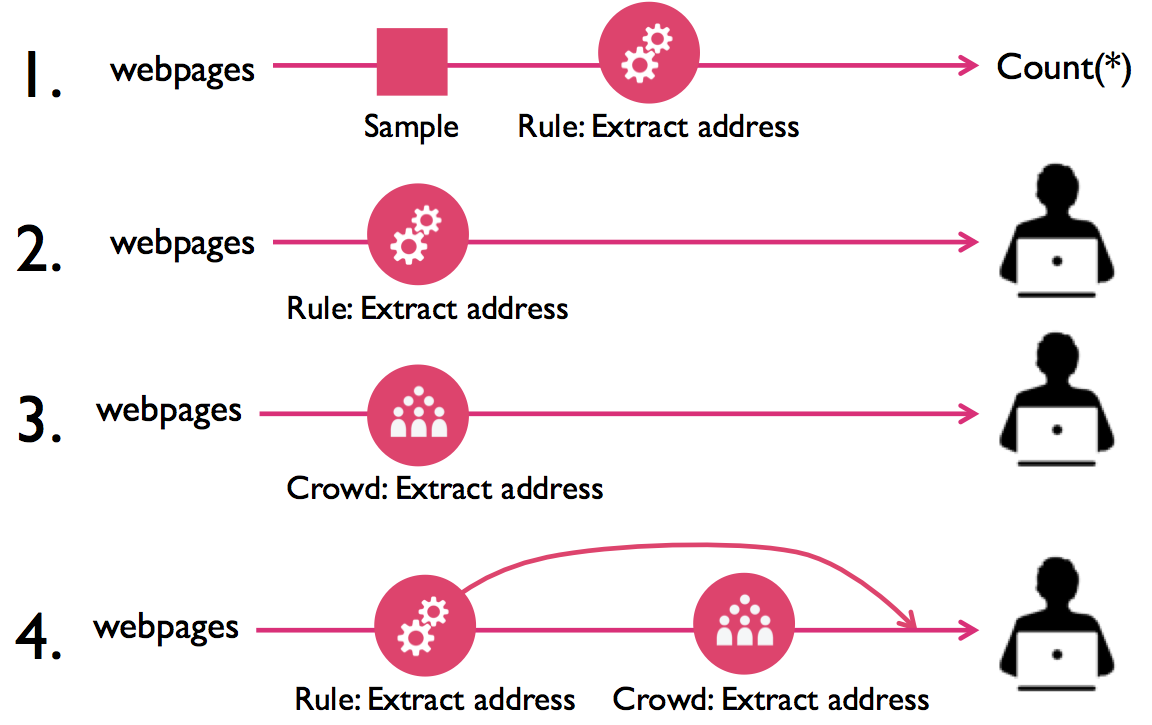
\includegraphics[width = .4\textwidth]{figs/lifecycle.png}
\vspace{-0.4cm}
\caption{Example iterations on the design of the portion of a cleaning plan that extracts restaurant addresses from their unstructured webpages.  
1) An exploratory plan that uses a sample to evaluate a simple address extraction method.
2) A plan that applies the method to the entire dataset. The quality is unsatisfactory. 
3) An alternate plan that uses manual crowd extraction. The quality is now high, but the crowd-based extractor is slow. 
4) A hybrid plan that sends only difficult webpages to the crowd, maximizing accuracy without sacrificing latency.}
\label{fig:ex-plan}
\vspace{-0.6cm}
\end{figure}
% why feedback loops exist/are important (cite Joe’s shit in the past 3 years, blinkdb, etc.). highlight domain specificity. Large variety of data cleaning tasks

%
% General comment that data cleaning is important:
%
The ease of acquiring and merging many large-scale data sources has led to a prevalence of dirty data.
Unfortunately, blindly using results that are derived from dirty data can lead to hidden yet significant errors in modern data-driven applications, so data must be cleaned before it is used.
But because data cleaning is often specific to the domain, dataset, and eventual analysis, analysts report spending upwards of 80\% of their time on problems in data cleaning~\cite{kandel2012}.
The analyst is faced with a breadth of possible errors that are manifest in the data and a variety of options to resolve them.
She must go through the cleaning process via trial and error, deciding for each of her data sources what to extract, how to clean it, and whether that cleaning will significantly change results.

Data cleaning is inherently iterative and Figure~\ref{fig:ex-plan} shows a common progression for the development of a data cleaning plan, in this case the extraction of a restaurant's address from its unstructured webpage.
While this operation can easily be represented at a \textit{logical} level by its input and output schema, there is a huge space of possible \textit{physical} implementations of the logical operator. 
For example, extraction could be rule-based, rely on structured learning, ask crowd workers to extract the desired data fields, or some combination of all three.
Even after selecting (say) a crowd-based operator, many parameters might influence the quality of the output data or the speed and cost of cleaning it: the number of crowd workers who vote on the extraction for a given webpage, the amount each worker is paid, etc.
A priori, a data analyst has little intuition for what physical plan will be optimal in this large space.

Note that in the evolution of the data cleaning plan in Figure~\ref{fig:ex-plan}, our data analyst needed to make many decisions manually about the choice of physical operators by reasoning about their latency, accuracy, and cost. 
Making the wrong decision, for example using the crowd when it only marginally improves accuracy, can be very costly.
A general, scalable, and interactive system that supports rapid iteration on candidate plans would greatly aid this process.

%The prevalance of data cleaning systems in both the research and industrial communities --
%Corleone does blah, XXX addresses blah. Nadeef does blah -- speak to the importance of a
%data cleaning framework as part of the modern big data ecosystems. \ewu{include open access of data in argument?} \jn{We also need to take a look at data cleaning systems in industry. }


% why existing systems suck aka related work
% 1. have slow feedback loops (dataset-dependence, …)
% 2. solve very specific data-cleaning tasks
%Since the beginning of data management, systems have been explored by both the research and industrial communities to improve data cleaning efficiency and quality.
Existing systems seldom address the end-to-end iterative data cleaning process described above.
Extract-transform-load (ETL) systems~\cite{informatica,talend,apachefalcon} require developers to manually write data cleaning rules and execute them as long batch jobs, 
and constraint-driven tools allow analysts to define ``data quality rules" and automatically propose corrections to maximally satisfy these rules \cite{DBLP:conf/sigmod/DallachiesaEEEIOT13}.
Unfortunately, neither provide the opportunity for iteration or user feedback, inhibiting the user's ability to rapidly prototype different data cleaning solutions.
Projects such as Wrangler~\cite{wrangler,trifacta} and OpenRefine~\cite{openrefine} support iteration with spreadsheet-style interfaces that enable the user to compose data cleaning sequences by directly manipulating a sample of the data and applying these sequences to the full dataset.
However, they are limited to specific cleaning tasks such as simple text transformations, do not support crowd-based processing at scale, and cannot incorporate user feedback to optimize the physical implementation of the data cleaning sequences.
Crowd-based~\cite{gokhale2014corleone,stonebraker2013data} systems have been proposed to relieve the data cleaning analyst of the burden of rule specification or manual cleaning, but are usually specific to a single cleaning task (e.g.,~\cite{gokhale2014corleone,park2014crowdfill,eracer,chen2014integrating}), preventing end-to-end optimization of the entire cleaning plan.
These existing limitations suggest the need for a system that is general enough to adapt to a wide range of data cleaning applications, scales to large datasets, and natively supports fast-feedback interactions to enable rapid data cleaning iteration.

In this paper, we introduce \sys, a system designed to support the iterative development and optimization of data cleaning plans end to end.
\sys allows users to specify declarative data cleaning plans composed of rule-based, learning-based, or crowd-based operators, then iterate rapidly on plans with cost-aware recommendations for improving the accuracy or latency of a plan.
The effects of a plan can be viewed early using sampling and approximate query processing techniques~\cite{wang1999sample}.

Supporting these capabilities requires a combination of careful engineering 
as well as tackling several research challenges:

\squishlist
\item \textbf{Sampling}: We provide sampling as a first-class logical operator for data cleaning plans that tolerate approximation, and use it to speed up iteration on early-stage plans.

\item \textbf{Recommendation}: We recommend cost-aware changes to in-flight cleaning plans that allow users to trade off accuracy and latency, and provide efficient mechanisms for implementing recommended changes without re-executing the plan on already cleaned tuples.

\item \textbf{Crowd Latency}: We leverage techniques for straggler mitigation~\cite{venkataraman2014power} and model crowd worker speed and accuracy to reduce the (often rate-limiting) latency of crowd data cleaning, consistently retrieving results in seconds rather than hours.
\squishend

In our demonstration, we will run an entity resolution plan on two restaurant datasets, and
show how \sys can be used to 1) specify, modify, and execute a data cleaning plan,
2) quickly clean a sample to characterize how a plan is performing, and
3) observe the same cleaning plans running on multiple datasets.
Users can execute plans over a live crowd that uses the audience as workers, or a simulated crowd
that uses pre-collected crowd responses. The dashboard (Figure~\ref{screenshot}) also provides a live inspection
interface to view the status of the cleaning plan as it executes.

\vspace{-0.2cm}
%Our contributions/requirements
%different ways to tighten the feedback loop:
%end-to-end latency/cost (operator optimization)
%looking versus touching
%Adding introspection (more points of observation)
%hot-swapping (more points of changing plans)
%We have built an end-to-end data cleaning framework with these requirements in mind. (... things we do …) (... engineering contributions …).
%In this demonstration, we highlight the benefits of improving feedback loops for data cleaning using X datasets by optimizing a data cleaning pipeline for one data set/cleaning task, then quickly fitting the pipeline to another dataset.


\if{0}

\jn{Honestly, I didn't quite buy declarativity of the system. In my opinion, data cleaning is so domain specific. It's hard to make it declarative. For a given domain, people may need to write their own data cleaning system. There is a lack of a data cleaning framework that they can build based on. This motivates us to develop such framework. 


We analyze a large variety of domain specific data cleaning systems, and identify several key components: declarative data cleaning operators (e.g., similarity joins), active learning, and crowd/expert sourcing platforms that they require. In our framework, we abstract these components, and implement them in a general way. 

We mainly address two challenges: extensibility and scalability. For the former one, we came up with a nice data-cleaning pipeline API, which people can easily use to compose their own data cleaning tasks. For the latter one, we address it in two aspects: Sampling + Asynchrony.}

\ewu{That's fair, will need to address why a framework is necessary and what benefits it provides.  I think a framework is the correct pitch, hard to sell a set of operators.  Are the above challenges -- extensibility and scalability -- actually difficult?  Worried it's straightforward application of existing techniques.}



In contrast, our work is based on the observation that the majority of data cleaning workflows
can be decomposed into a small set of logical operations (in addition to traditional database operators):
filter based on constraints, extract new fields from existing data, and a similarity join to match
similar or duplicate records. \ewu{quickly validate why this observation holds.} \jn{Yes! I also found that Sec 2.3 has more operators than you describe here.}  
By designing a system around these core operators, we can provide a vast library of physical  
data cleaning operators that span the range of algorithmic, machine learning, and human computation-based
implementations that are necessary practical data cleaning pipelines.   \ewu{Describe live inspection as 
a core feature or is it too easy?}

Designing such a system requires tackling several design challenges:

\begin{enumerate}
\item Speed
\item Quality
\item API Design/extensibilty
\end{enumerate}



We have implemented an initial version of \sys on top of the AMPLab Spark stack, which provides us 
with access to its advanced distributed processing and machine learning features.  Our goal for the current
version is to implement the core mechanisms for declarative specification of the
data cleaning pipeline, solidify the API design, and incle support for, and implementations of,
multiple classes of physical data cleaning operators.


\fi



\if{0}

Cleaning, pre-processing, and formatting data is a required first step in any data analytics pipeline.
However, despite this importance, large-scale data analytics platforms such as Spark or Hadoop lack integrated data cleaning frameworks.
There are a few challenges in building a general purpose data cleaning framework: (1) data cleaning is often
domain specific and requires specialized software targeted at one or a handful of data sources \cite{wang1999sample}, (2) data cleaning is often 
expensive as it increasingly involves human effort via crowdsourcing or experts \cite{DBLP:conf/sigmod/GokhaleDDNRSZ14}, and (3) learning how to clean dirty data from examples
is often hard without a greatly restricted set of operators \cite{DBLP:conf/uist/GuoKHH11}.

We address this problem in \projx by designing a Spark library of composable and scalable data cleaning primitives.
\projx abstracts the logical data cleaning operators: Extraction, Similarity Join, Filtering, from the physical implementation i.e, Rule, Crowd, or Machine Learning.
We interface these primitives through a DSL with which a user can build data cleaning operators that suit their needs.
\projx provides transparent optimizations for each of the components and their composition.
In this demonstration proposal, we present \projx and highlight some of its key features.
While there are many existing systems that do one aspect of data cleaning and transformation (e.g Entity Resolution or Extraction), 
many real world data cleaning tasks have multiple types of errors.
Composing disparate systems can lead to complex code and inefficiencies at scale.
With \projx, we hope to design a set of optimized composable primitives that span a large space of data cleaning tasks.

The first key feature of \projx is that it provides optimized distributed implementations 
of the physical data cleaning operators.
For example, a key step in many deduplication algorithms is a Similarity Join which finds all pairs of records that are within some similarity threshold.
A naive implementation of a Similarity Join would apply a similarity function to all pairs of records.
However, in \projx, we provide optimized implementations of certain common similarity functions (e.g Jaccard, Edit Distance, etc.) that allow for 
a combined broadcast join and prefix filtering which intelligently skips pairs of records using a broadcasted inverted index.

Another feature of \projx is managing the latency and the scale problems of crowd-based data cleaning. 
Crowdsourcing is increasingly prevalent in data cleaning, and \projx provides physical crowd-based implementations
of the logical operators.
However, crowds work at a different latency and scale point in comparison to distributed analytics platforms.
To address the latency problem, we build asychrony into the system.
The user can query intermediate results at any time as crowd responses stream in.
To address the scale issue, \projx provides sampling primitives.
The glue that ties all of the crowd components together is a Machine Learning technique called Active Learning.
As we collect more and more crowd responses, we learn a model that predicts these responses to apply it on the uncleaned data.
Active Learning selects the most informative questions to ask the crowd.

Finally, \projx provides an approximate query processing (AQP) framework.
With slow asynchronous data cleaning algorithms as in crowdsourcing, we need 
to define clear semantics for the intermediate results.
Our AQP framework uses the algorithms proposed in \cite{wang1999sample}, to estimate and bound early results.
It is also common for data scientists to prototype expensive data cleaning pipelines on samples and AQP allows quick evaluation of
aggregate query results on a cleaned sample.

\subsection{Demonstration Scenario}
\reminder{TODO}

\fi




\if{0}
Consider for example, the ability to rapidly understand the types of errors that are present, as well as prevalance of 
these errors is cruicial.



Before an organization can use a new dataset as part of their analysis pipeline
(e.g., to build complex learning models or answer analyst queries)
the errors in the dataset need to be removed in order to ensure accurate conclusions.  

Modern data-driven organizations rely on the ability to ingest and generate large data sets from 
disparate sources, and combine the data together to build complex models or answer analytical questions.  
For example, a restaurant review website may collect restaurant listings by scraping data from webpages or purchasing them from external sources, and
restaurant visitation information for sources such as OpenTable or FourSquare, and aggregate the data to
model user eating habits.  
The set of cleaning tasks necessary for each of these data sources is highly domain and application specific,
and oftentimes the developer is concurrently trying to clean the data source as well as understand its properties.


Oftentimes, these data sources have data quality issues that require a complex data cleaning pipeline -- 
e.g., data extraction, re-formatting, identification and fixes of missing or incorrect values,
and removal of redundant information -- before the data is useable by downstream processes.
Data sources are often domain specific and new for the data analyst, 
As datasets continue to grow, and organizations make use of mure and more datasets, the ability to
rapidly clean the data is more important.  
\fi

% !TEX root = demo.tex
\section{System Architecture}

In this section, we provide a brief overview of the \sys system and its APIs.
Figure~\ref{fig:arch} depicts the system architecture.

\begin{figure}[t]
\centering
\vspace{-0.5cm}
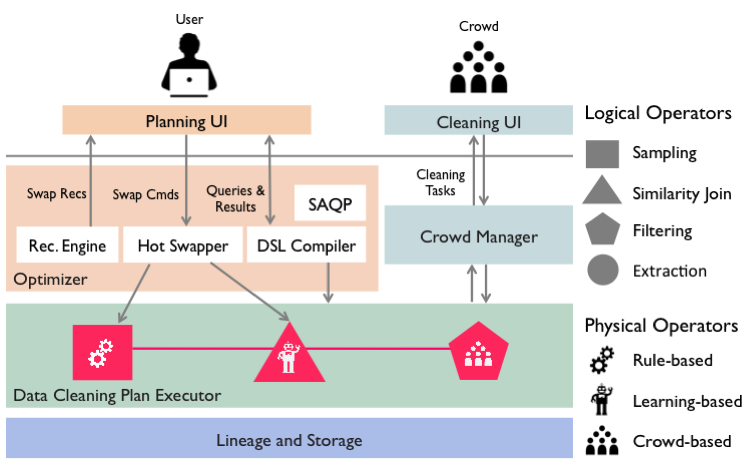
\includegraphics[width = .5\textwidth]{figs/architecture.png}
\vspace{-0.6cm}
\caption{\sys system architecture, with an example entity resolution plan.}
\vspace{-0.7cm}
\label{fig:arch}
\end{figure}

\subsection{Architecture Overview}
The \sys architecture provides UI, language, and systems tools for building data cleaning plans.
Users interact with the system through the \textbf{Planning UI}, which allows them to compose data cleaning workflows from modular operators.
These workflows are represented as expressions in our data cleaning language (section~\ref{sec:dsl}), then synthesized as data cleaning plans by our \textbf{DSL compiler}.
As the \textbf{Data Cleaning Plan Executor} executes the compiled plans, users can interact with the plans via tight feedback loops in two ways.
First, users can issue queries to the \textbf{SAQP module} and observe approximate results based on the data that has been cleaned thus far.
Second, the \textbf{Recommendation Engine} displays a set of suggested modifications to the active cleaning plan (for example, making a similarity join more permissive) in the \textbf{Planning UI}, and users can update the data cleaning plan in-flight by accepting a suggestion and using the \textbf{Hot Swapper} to modify components of the pipeline.
Intermediate results and cleaned data are maintained in a \textbf{Lineage and Storage engine} that tracks each tuple's lineage in order to enforce the semantics of hot-swapping correctly on in-flight tuples.
Logical cleaning operators may have a number of physical implementations (section~\ref{sec:operators}).
Automated rule-based or learning-based operators leverage Spark and MLLib for efficient distributed computation, and operators that require human intervention call out to \sys's \textbf{Crowd Manager} API, which renders data cleaning tasks and displays them to crowd workers from multiple crowds (e.g., Amazon Mechanical Turk) in a web-based \textbf{Cleaning UI} for processing.

\subsection{Cleaning DSL}
\label{sec:dsl}
We provide a language for specifying the composition of data cleaning operators.
The logical operators define the input and output behavior of the operation and 
the physical operators specify the implementation.
The general syntax of this language is:
{\scriptsize
\begin{lstlisting}
<logical operator> on <relations>
  with <physical operators> , <params>
\end{lstlisting}
}

These expressions are composable. For example, the following represents the data cleaning plan in Figure~\ref{fig:arch} (an entity resolution plan):
{\scriptsize
\begin{lstlisting} 
Filtering on (
    SimilartyJoin on (
        Sampling on BaseTable
        with Uniform)
    with Jaccard, thresh=0.8) 
with CrowdDeduplication, numVotes=3
\end{lstlisting}
}
Additionally, \sys provides integration of our DSL with Scala/Apache Spark, allowing SchemaRDDs (Spark RDDs with additional schema information) to serve as base tables in expressions.

\subsection{Cleaning Operators}
\label{sec:operators}
\sys supports a small set of operators that can express a wide variety of common data cleaning workflows. 
For example, the pipeline depicted in Figure~\ref{fig:arch} performs crowd-based entity resolution: the similarity join operator generates candidate tuple pairs (the \textit{blocking} step), and the crowd-based filter operator uses humans to identify duplicates from the candidates (the \textit{matching} step). 
Additional operators include Extraction and Sampling.

Individual logical operators have multiple physical implementations, each with its own cost, latency, and accuracy profile. 
For example, crowd-based implementations tend to be high cost, high latency, and high accuracy, whereas rule-based implementations tend to be low cost, low latency, and low accuracy. 
The \texttt{with} clause of our data cleaning language allows users to explicitly specify desired physical operators, and \sys's recommendation engine provides actionable suggestions for modifying the pipeline to navigate the tradeoff space.






%\subsection{Logical Operators}
\projx specifies three logical operators: Extraction, Filtering, and Similarity Join. 
\sanjay{In depth why these operators are {\it sufficient}.}

For performance (or some other reason), we support several additional
logical operators tha enable optimization: Sampling, Async, and Transitive Closure.
The composition of these operators support a variety of data cleaning
operations. 
For example, a deduplication task can be expressed as a Similarity Join to pair similar records
together and then a filtering task to remove false positives.
These logical operators specify the input and output data schema and allow us to compose operations.


\vspace{0.5em}

\noindent \textsf{SimilarityJoin(R,S,$\phi$, $t$)}: For a given relations $R(a_1,...,a_l)$ and $S(b_1,...,b_k)$, a similarity function $\phi$, and a threshold $t$, the similarity join of R and S is defined by:
\[
\{ (r,s) \in R \times S \text{ s.t } \phi (r,s) \ge t \}
\]

\vspace{0.5em}


\noindent \textsf{Filter(R, $\rho$)}: For a given relation $R(a_1,...,a_l)$ and a boolean condition $\rho$, return $R' \subseteq R$ that satisfies $\rho$.

\vspace{0.5em}

\noindent \textsf{Extract(R, a, $\epsilon$)} For a given relation $R(a_1,...,a_l)$, a attribute $a$, and an extraction function $\epsilon$, apply $\epsilon$ to every $R(a)$ returning $\epsilon(R(a)) = (v_1,...,v_k)$. The result relation is:
\[
R(a_1,...,a_l,\epsilon(R(a)))
\]

\noindent \textsf{Sample(R, $m$)}: For a given relation $R(a_1,...,a_l)$ and return $R' \subseteq R$ such that each $r \in R$ is in $R'$ with probability $m$.

\vspace{0.5em}

\noindent \textsf{Project(R, $p_1,...,p_k$)}: For a given relation $R(a_1,...,a_l)$ and return $R(p_1,...,p_k)$.

\vspace{0.5em}

\noindent \textsf{TransitiveClosure(R,$f$)}: For a given relation of pairs of rows from the same base relation, e.g the result of a self-Similarity Join, $R(a_1,...,a_l, b_1,...,b_l)$ return the transitive closure of the relation $S(a_1,...,a_l)$. $f$ is called a cannonical representation function, this takes a set of associated records and returns a single record that is designated as the canonical representation.






%\section{Physical Operators and Implementation}

For each of the logical operators there are different physical implementations.
We do not currently select the appropriate physical operator and the user has to specify this.
We do, however, set sensible default parameters for each of the physical operators.
In \projx, there are three broad categories of physical operators: Automated, Crowd, and Learning.
An automated physical operator is conceptually the same as a SQL user defined function, while a crowd operator uses a microtask platform.
A learning operator takes in training examples (whether crowd or ground truth) and learns an automated operator.
We describe each below.

\ewu{below are straightforward physical implementations of the
logical operators.  Is there anything interesting to say about their
design or a specific physical operator?}

\team{How do we know when transitive closure/any of the physical operators can be safely applied?  Are there properties of the physical ops that could tell us?}


\subsection{Similarity Join} 
\projx provides a library of the following commonly used similarity functions: \textsf{JaccardSimilarity}, \textsf{DiceSimilarity},
\textsf{CosineSimilarity}, \textsf{OverlapSimilarity}, and \textsf{EditDistance}.
The user can select one of these similarity functions.
A naive implementation of a Similarity Join is to take the cartesian product and then filter all pairs of record of similarity greater than $t$.
However, the implemented similarity functions are all symmetric and the similarity function is maximized when $r = p$.
So it suffices to compute a similarity $\theta$-join instead of the full Cartesian product.
We can further add an optimization called prefix filtering to further reduce the number of similarity function evaluations.
In prefix filtering, we prune pairs that cannot possibly meet the threshold $t$ based on the number of tokens that overlap which can be determined with an inverted index.


\subsection{Extraction}
We implement basic automated extraction libraries including delimited splitting and regular expression methods.
However, extraction is a task that is well suited for crowd sourcing.
We provide a parametrized interface that allows the user to specify an extraction attribute, a formatting question, and request data from the crowd.
In Figure \ref{fig:entry}, we illustrate an example of this task.

\begin{figure}[ht!]
\centering
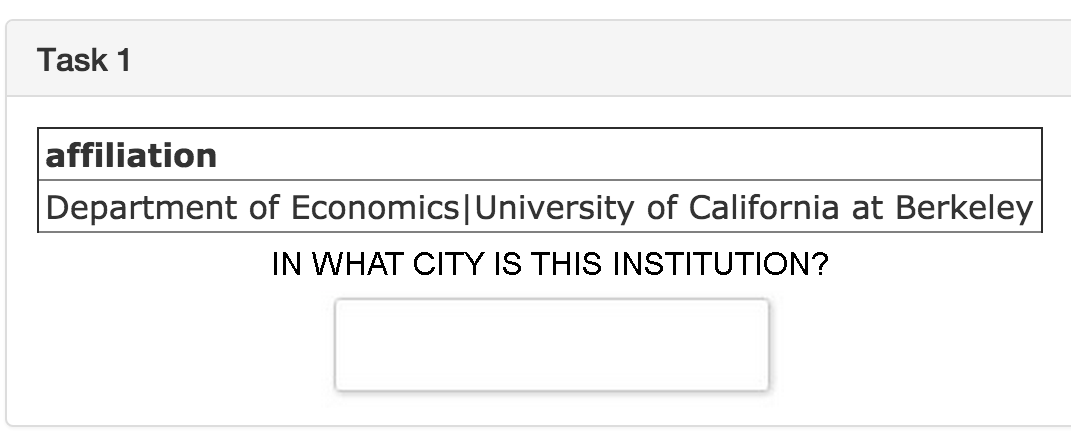
\includegraphics[scale=0.25]{figs/entry.png}
\caption{Example of the Extraction Crowd Interface. \label{fig:entry}}\vspace{-.5em}
\end{figure}

\subsection{Filtering}
We provide an interface for a user defined predicate.
However, as with extraction, filtering has many opportunities for crowdsourcing.
For a filtering operation, the crowd response is binary in contrast to Extraction.
We provide crowd templates for two types of filtering tasks.

\noindent\textbf{Condition Checking: } Given a single record, a crowd worker indicates if it satisfies some condition. In Figure \ref{fig:condition},
we illustrate an example condition checking task.
\begin{figure}[ht!]
\centering
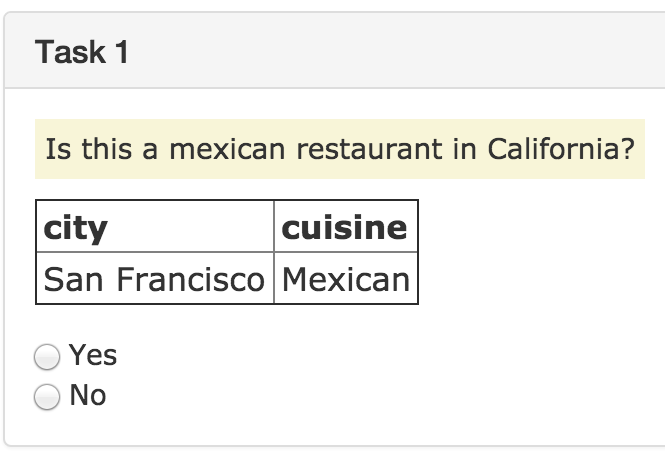
\includegraphics[scale=0.25]{figs/condition.png}
\caption{Condition checking is one variant of the filtering crowd interface.\label{fig:condition}}\vspace{-.5em}
\end{figure}

\noindent\textbf{Pair Comparison: } Given a pair of records, a crowd worker indicates if they are the same or are different. In Figure \ref{fig:pair},
we illustrate an example pair comparison task.

\begin{figure}[ht!]
\centering
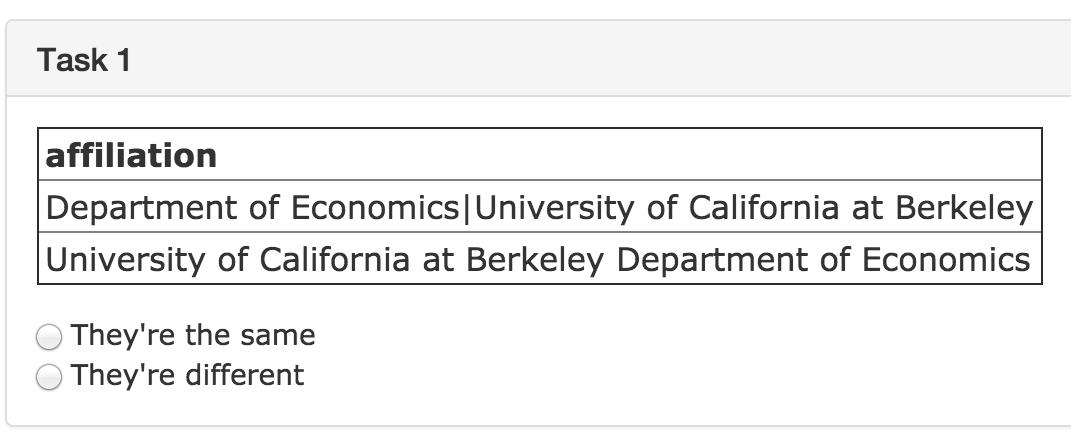
\includegraphics[scale=0.25]{figs/pair.png}
\caption{Pair comparison is the other variant of the filtering crowd interface.\label{fig:pair}}\vspace{-.5em}
\end{figure}



\subsection{Extended Operators}

\subsubsection{Sampling}
\projx provides different variants of uniform sampling.
We provide Bernoulli sampling (in which flips a ``biased coin" for each row) or hash sampling (which hashes an attribute).
Hash sampling allows for joining sampled relations with foreign key relationships.
On the other hand, Bernoulli sampling is less sensitive to skews and leads to more consistent sample sizes.

\subsubsection{Transitive Closure}
Similarity Joins can create issues with transitivity.
For example, rowA might be similar to rowB and rowB might be similar to rowC, but rowA might not be similar to rowC.
We can associate these relationships with edges in a similarity graph.
Then to enforce transitive closure, we solve a connected components problem.
We apply a distributed using a distributed gather-apply-scatter connected components algorithm in the Spark-integrated graph library GraphX.




% %!TEX root = demo.tex
\section{Logical Operators}


\ewu{INSERT: implementation in Spark}

Now, we discuss the logical operators and their parameterization defined in \projx.

\vspace{1em}


% !TEX root = demo.tex
\section{Research Challenges}
To support evolving data quality needs, there are three main research challenges in \sys: (1) sampling, (2) recommendation, and (3) crowd sourcing.

\subsection{Sampling}
In prior work, we explored the problem of estimating aggregate query results over dirty data ~\cite{wang1999sample}.
In SampleClean \cite{wang1999sample}, we found that aggregate queries can often be answered with very high accuracy (i.e 99\%) with only a small fraction of clean data, and we can clean just enough for the application's data quality requirements.
In the context of the iterative design, data analysts often run aggregate queries, e.g., count the number of Chinese restaurants, on a new data source to assess the quality of the data.
In \sys, we implement sampling as a logical operator that can be used for quickly prototyping and optimizing workflows on samples of data and then transferring these optimizations to full datasets.
There are many additional research opportunities with sampling.
For example, sampling allows for quick introspection of otherwise opaque operators, such as testing the quality of a crowd with a small set of records.
We also build a significance testing framework to allow users to declare aggregate queries of interest and notify them when a change to 
a plan has a statistically significant effect.

\subsection{Recommendation}
Our next research challenge is to recommend changes to a data cleaning plan based on user feedback. 
The user can inspect the output of an operator and identify result tuples that are incorrect. This feedback is operator specific. For example, in a Similarity Join the user can mark false positives (matched pairs that should not be similar) and false negatives (unmatched similar pairs) and in an Extraction the user can mark incorrect attribute values. 
We highlight two key challenges: generating recommendations and applying the recommendations mid-execution.

\vspace{.25em}

{\noindent \bf Recommendations:} There are three types of recommendations: (1) parameter change, (2) operator replacement, and (3) operator addition.

\textit{Parameter Change.} Many of the physical operators in \sys have tunable parameters, whose values is often very dataset-specific, and the user feedback gives us a way to evaluate the quality of the initial parameter choice. 
For example, Similarity Joins have a similarity threshold and a similarity function. 
Increasing this threshold reduces the selectivity of the join, and \sys chooses a threshold that maximizes the F1-score. 

\textit{Operator Replacement.} 
\sys recommends changes to these physical operators when the user indicates that they are not satisfied with the output.
For example, we can use the user feedback as training examples in our learners as an estimate of the crowd performance.
This allows us to estimate the value of replacing the physical operator with an active learning variant.
Additionally, we can try different variants of automated operators to test how accurate they are with respect to the user feedback.

\textit{Operator Addition.}  There are also cases where we may want to add another physical operator, while still preserving the logical input-output behavior of the workflow.
It is common in extraction tasks to have most records accurately extracted with an automated extractor but only a small subset requiring additional inspection. 
For these cases, we can add a crowd-based Filter operator to separate these examples for additional cleaning.

\vspace{.5em}

{\noindent \bf Dynamic Modification:} To be able to quickly modify cleaning plans after recommendations, we explore ways to intelligently re-use computation. Because cleaning can be time-consuming, it is inefficient to 
restart the plan every time the user wants to make a small change.
We design a framework for \emph{hot swapping} plan operators that re-uses existing results while ensuring that the output of the swapped plan is the same as if the new plan had been run from the start.

\textit{Caching} allows for result re-use if a downstream operator is modified or added.
If the system has sufficient memory, then we can cache all of the intermediate results. 
However this is not always possible, and the key challenge is to select which results to cache.
To do this, we have to integrate the caching framework with our recommendation engine.
When we make a recommendation for a change, we must cache the preceding operator. 

\textit{Lineage} allows us to understand how results change if upstream operators are modified.
For example, decreasing a similarity join threshold increases the number of output pairs, but adding an additional filtering step 
reduces the number of output tuples. The key property here is monotonicity, and some types of monotone \textsf{Filter} and \textsf{SimilarityJoin} are data cleaning analogs for a Select-Join relational algebra.
We can therefore model upstream hot-swapping as an incremental view maintenance problem and update the 
final result based on the insertion or deletion of tuples earlier in the plan.

\iffalse
\vspace{.5em}

{\noindent \bf Cost Estimates:} Of course, changing plans when using crowdsourcing may significantly change its cost.
For every recommendation, we estimate the number of additional tuples processed by the crowd operators and provide 
the user with an estimated cost.

\fi

%\subsubsection{Dynamic Modification}
%The next category of optimizations happen at the plan-level, i.e., the sequence or execution pattern of the operators.
%We highlight two challenges: allowing users to see early results, and allowing users to modify plans mid-execution.
%\vspace{.3em}
%{\noindent \bf Asynchronous Data Cleaning:} To provide fine-grained feedback during a data cleaning process, our system executes data cleaning operations asynchronously. Tuples are processed in a streaming fashion by each of the operators in the plan and the intermediate results are persisted, allowing users to query the results at any time. Thus, at any time, the user can get a ``best effort" query result.
%\vspace{.3em}


\vspace{-0.2cm}
\subsection{Crowdsourcing}
\vspace{.2em}

%{\noindent \bf Sampling:} One way to reduce operator latency is to reduce the number of tuples each operator processes.
%In \sys, sampling is a first-class logical operator that can be used for quickly prototyping and optimizing workflows on samples of data and then transfering these optimizations to full datasets.
%Sampling allows for quick introspection of otherwise opaque components, such as testing the quality of a crowd with a small set of records.
%\sys also provides the statistical tools to extrapolate (with confidence intervals) the insights learned on a sample.
%The problem of estimating aggregate query results over dirty data has been investigated in prior work~\cite{wang1999sample}, 
%addressing the challenge that data cleaning may change the underlying statistics of a sample.
%In this work, we build on these results to allow users to declare aggregate queries of interest and notify them when a change to 
%a plan has a statistically significant effect.

%Recently proposed, sample-based query processing methods for dirty data can help inform users the changes about the statistical significance of 
%changes made to the data.
%For example, suppose one collects a restaurant dataset, and runs some aggregation queries on the dataset, e.g., computing the number of the restaurants in San Fransisco and getting a query result of 12000. 
%But, when looking at the dataset, she finds that there are many duplicate restaurants in the dataset, and some restaurants' locations are misspelled (e.g., S\underline{e}n Fransisco). She can use our system to create a sample of the data, and then apply a data cleaning procedure to the sample. 
%After the sample is cleaned, our system can estimate the impact of data cleaning on her original query results, and return her corrected answers with confidence intervals, e.g., $5000\pm300$. Intuitively, this result means that if the same data-cleaning procedure is applied to the full dataset, the number of the restaurants in San Fransisco will be within $[4700, 5300]$. 

%\vspace{.5em}
%{\noindent \bf Crowdsourcing and Active Learning:} 
Working with crowds is inherently challenging: unlike with automated operators, the accuracy and speed of processing each tuple varies widely with the crowd worker assigned to it.
Completion time of an operator depends on the response times of individual workers, and on real-world crowdsourcing 
platforms, the distribution of response latencies is highly skewed; analogous to the straggler problem in distributed systems.
We address this problem by maintaining a pool of high-speed, high-quality crowd workers and develop task routing strategies 
that can avoid assigning tasks to slow workers and leverage redundancy to significantly reduce the time that is required to clean 
data with the crowd. Additionally, active learning techniques reduce the number of tuples that require crowd work to clean the
data.
Another challenge with crowd operators is that some workers may give inccorect responses.
We modify state-of-the-art quality control techniques for the active learning setting using redundancy and Expectation-Maximization based voting algorithms.
%Even cleaning a sample of data, data cleaning can still take a lot of time. This is especially true when it requires humans to clean the data. 

\vspace{-0.25cm}


\iffalse
\subsection{Research Challenges}

Architecturally, we separate crowd sourcing and automated data cleaning.
There is a crowd server that acts as a layer of indirection between the Spark codebase and crowd sourcing APIs.

\team{Describe Research Challenges.  To what extend can we actually do
optimization given the physical operators?  Unlike relalgebra, the physical operators here are
not interchangable!}



\subsection{Learning Parameters From Example}
In simple cases, it might be easy to use domain knowledge to select and tune physical operators. 
In more complex cases, it might be easier to specify a sample of dirty and clean data instead of the function.
It may also not be feasible to have the crowd clean the entire dataset.
In these cases, we want to learn a statistical model from which we can extrapolate those responses to the rest 
of the data.

In our current implementation of \projx, we pose this learning problem as classification problems.
In general, these parameter functions can be quite complex and this is a simplification of the learning problem.
The choice of classifier and featurization is upto the user. 
We currently support Support Vector Machines and Decision Trees with a featurization library that includes common text processing features.

\vspace{0.5em}

\noindent \textsf{Filter(R, $\mathcal{T}^+$, $\mathcal{T}^-$)}: Given a set of positive training examples $\mathcal{T}^+$ (i.e, $r$ that satisfy the condition) and
negative training examples $\mathcal{T}^-$ (i.e, r that do not satisfy the condition), we learn a classifier that predicts whether a record satisfies the condition. 

\vspace{0.5em}

\noindent \textsf{Extract(R, a, $\mathcal{T}$)} We restrict the learned problem setting to delimited extraction. Given a set of training examples $R(a)$ and the output $v_1,v_2,...,v_k$, we learn a classifier to predict which characters in $R(a)$ are delimiters based on the tokens in the string.

\vspace{1em}

To acquire the samples of clean data, uniform sampling may not be the best strategy.
For example, if there examples of dirty data are very rare, we will not be able to learn a model.
We implement a technique called Active Learning to sample.
Active Learning selects the most informative examples based on the current model so far.
We use an Active Learning algorithm called uncertainty sampling to do this.




\subsection{Inspection}

Data cleaning requires inspection -- user wants to see how the dataset
has been "cleaned"  through the pipeline.  What does that even mean?

\subsection{Dynamic Re-optimization}

Crowd means want to swap in or out operators at run time.


\subsection{Lineage}

\noindent\textbf{Lineage: }
We track the lineage of rows using a primary key.
Users are not allowed to modify this primary key with any operations.
This allows us to apply operations like transitive closure even after projection since we have a unique identifier for each row.

\vspace{0.5em}
\noindent \textbf{Example: } Suppose, we are interested in deduplication of unstructured data. Then, we could apply the following logical operations.
We first apply an \textsf{Extract} operation to extract the unstructured data into columns. If some of the columns are inconsistent in their representation,
we apply \textsf{Project} to those columns that are inconsistent. We can then take a \textsf{SimilarityJoin} to group rows that are similar, and finally
we resolve those differences with \textsf{TransitiveClosure}.
\fi



%% !TEX root = demo.tex
\subsection{Engineering Challenges}
In addition to the numerous research challenges, there have been substantial challenges in engineering \sys.
We highlight two key challenges: API design and Crowdsourcing.

\subsubsection{API Design}
Currently, there are many systems that address specific types of data error \cite{gokhale2014corleone,park2014crowdfill,eracer,chen2014integrating}, but it is often 
the case that data are corrupted in multiple ways.
Unfortunately, there is currently no interoperability between these systems, since some are constraint-based, some use generic crowd APIs, and others have custom crowd interfaces.
In \sys, we address this problem by designing an API that allows for the composition and optimization of data cleaning operators.
Many of the research challenges in \sys rely on clear specifications of the input and output behaviors of
individual data cleaning operators.
For example, Hot Swapping is only possible between two physical operators that have exactly the same input and output specification.
The engineering challenge is to retain modularity and extensibility while restricting operators.
We build a class hierarchy of data cleaning operators which through inheritance and parameterization specify clear input and output behaviors.

One draw back of an extensive API is that the choices may overwhelm a user.
Many of our API methods and classes come with inherited sensible defaults.
For example, if the user fails to completely specify the semantics of the similarity function through the API, 
the system will avoid optimizations and perform a naive Cartesian products and filtering.
These behaviors come naturally through the use of inheritance and polymorphism.

\subsubsection{Crowdsourcing Platform}
The second engineering challenge is designing a platform to serve crowd tasks.
Working with crowds is inherently challenging: unlike with automated operators, the accuracy and speed of processing each tuple varies widely with the crowd worker assigned to it.
We have developed a ``crowd manager" as a layer of indirection to support this complexity.
This component handles serving and processing crowd tasks and automatically uses our techniques for latency reduction as well as state-of-the-art quality control techniques using redundancy and Expectation-Maximization based voting algorithms.

The other benefit of a crowd manager is that it provides an abstraction layer over the varied APIs of Mechanical Turk, Crowd Flower, and others.
We leverage the fact that most crowd platforms serve tasks through a browser-based interface, generating tasks in the form of dynamic web pages and processing responses via AJAX callbacks to our own server.
As a result, tasks submitted to the crowd manager can be processed easily on a variety of different crowds including AMT, Crowd Flower, or a private ``Internal Crowd".
%\input{implementation.tex}
%\section{\projx DSL}
We design a DSL for the composition of data cleaning operations.
The general syntax of this language is:
\begin{lstlisting}
<logical operator> on <relations>
	with <physical operators> , <params>
\end{lstlisting}
In this section, we will highlight some key examples.
We have an additional operator \textsf{Async} which designates the 
execution of the operator to be synchronous or asynchronous.

\subsection{String Extraction}
One of the most common data cleaning operations is delimited extraction.
In our DSL, this can be expressed in the following way:
\begin{lstlisting}
Extract on Data
with Split, `,',
cols=[col1, col2]
\end{lstlisting}

We can also use a format string:
\begin{lstlisting}
Extract on Data
with FmtString, `%s:%s',
cols=[col1, col2]
\end{lstlisting}

\subsection{Crowd Entity Resolution}
Crowd-based techniques for entity resolution are increasingly popular e.g Corleone \cite{DBLP:conf/sigmod/GokhaleDDNRSZ14}.
We present an example of expressing a crowd-based technique for entity resolution with the DSL.
Let us suppose we have a database of addresses that we want to deduplicate.
The first step is to group similar rows together and a good similarity metric to use is JaccardSimilarity.
\begin{lstlisting}
SimilarityJoin on Data
with Jaccard, thresh=0.8
\end{lstlisting}
The next step is to filter these pairs using the crowd. 
However, since most pairs will not be duplicates we want to use Active Learning.
Furthermore, since the crowd might be slow, we can add asynchrony.
\begin{lstlisting}
Filter on
( 
 SimilarityJoin on Data
 with Jaccard, thresh=0.8
)
with Crowd, Active, Async
\end{lstlisting}
To resolve the changes, we apply transitive closure at the end that takes the 
longest address:
\begin{lstlisting}
TransitiveClosure (
 Filter on
 ( 
  SimilarityJoin on Data
  with Jaccard, thresh=0.8
 )
 with Crowd, Active
) with Longest
\end{lstlisting}




% !TEX root = demo.tex
\section{Demonstration}
In this section, we detail the proposed demonstration.
The objective of this demonstration is to illustrate 
how \sys enables the rapid iterative construction of data cleaning plans
and the ability to transfer workflows between similar dirty datasets.

\subsection{Datasets}
In the demo, we will consider cleaning workflows on three different datasets.
The first dataset contains 858 Zagat reviews\footnote{\scriptsize{ \url{cs.utexas.edu/users/ml/riddle/data/restaurant.tar.gz}}},
each tagged with the cuisine of the restaurant reviewed (e.g. ``Chinese" or ``French").
The second dataset, which is similar to the first, is from Yelp \footnote{\scriptsize{\url{https://www.yelp.com/academic_dataset}}} and contains 58,127 restaurant records that are also tagged with a category.
The third dataset consists of $3,049,914$ records of liquor sales from the state of Iowa\footnote{\scriptsize{\url{data.iowa.gov/Economy/Iowa-Liquor-Sales/m3tr-qhgy}}}, including the store where the purchase occurred and the items and cost of the purchase.
In all three datasets, categorical columns are inconsistent across records (e.g. cuisine tags for ``Chinese" vs. ``Chinese Cuisine"), records are duplicated, and formatting errors abound. 
We will use \sys to resolve these errors using Extraction and Entity Resolution, then run aggregate queries over the cleaned datasets.

\begin{figure}[t]
\centering
 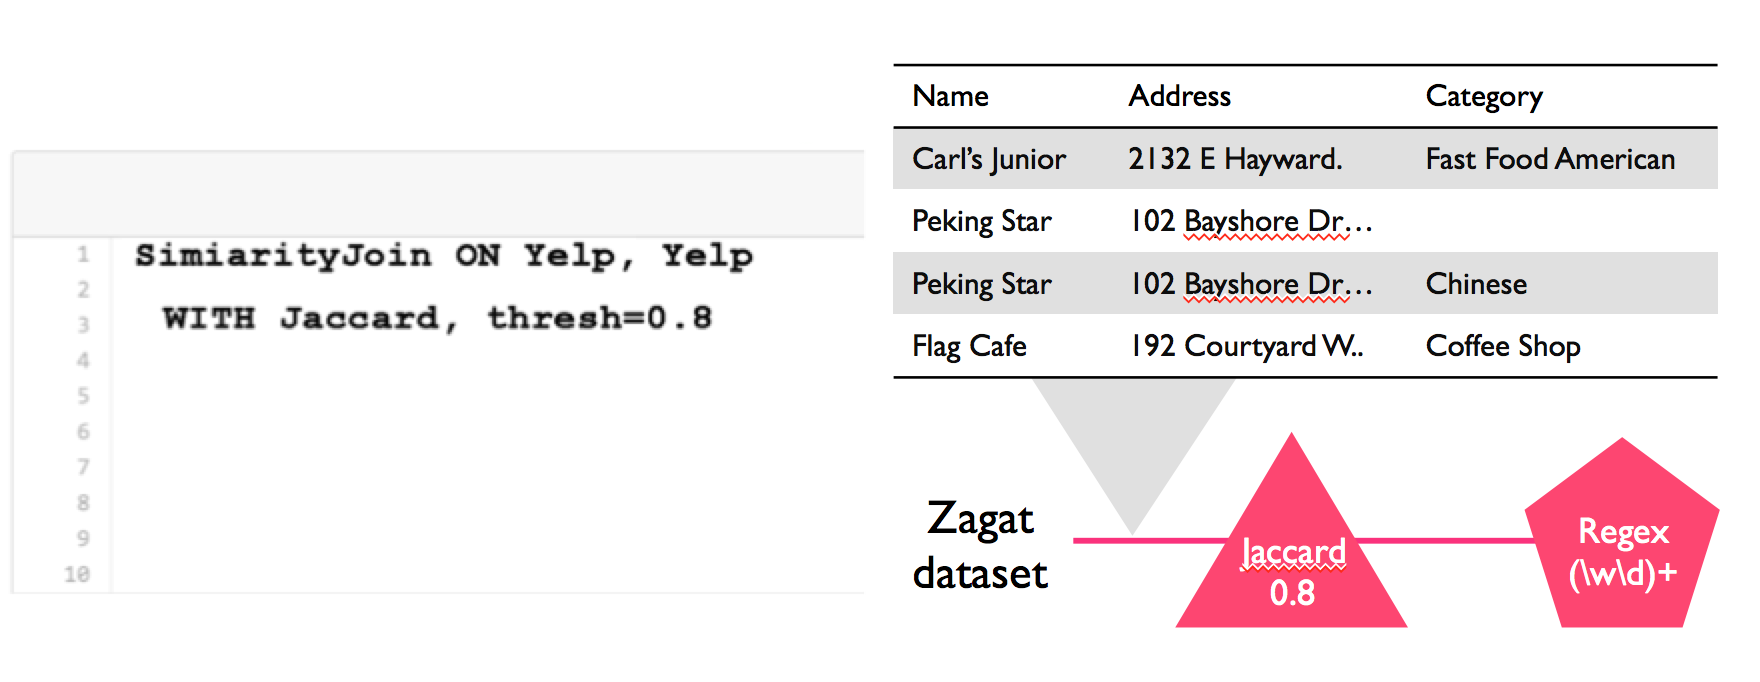
\includegraphics[width=\columnwidth]{figs/dashboard_screenshot.png}
 \caption{The dashboard contains both a visual interface and a text box to specify data cleaning operations. When the user is satisfied, she can run the plan and see the results on the right. \label{screenshot}}
\end{figure}


\begin{figure}[t]
\centering
 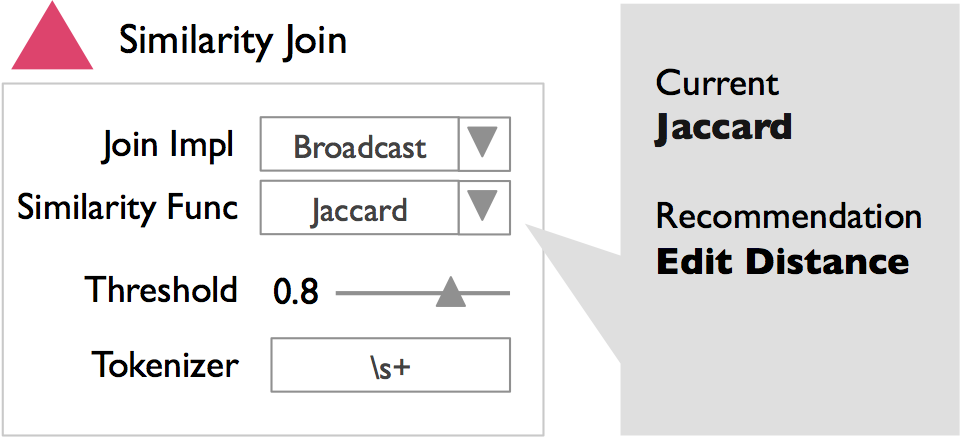
\includegraphics[width=0.8\columnwidth]{figs/dashboard_recsys.png}
 \caption{The operator view lists the parameters of an operator. Users can view recommended changes and modify parameters on the fly.}
 \label{screenshot-rec}
 \vspace{-0.4cm}
\end{figure}

\subsection{Demo Walkthrough}
Below, we detail the steps of the proposed demonstration.
A screenshot of the dashboard interface is illustrated in Figure~\ref{screenshot}.

\vspace{0.2em}

\noindent\textbf{Step 1: } Participants will select a dataset (e.g., the Zagat dataset), and load a pre-populated data cleaning plan and target query for it.
Participants must first extract the columns of the dataset into the proper schema using a regex-based Extraction.
Then, participants will be able to manually tune the Enity Resolution by choosing between Similarity Join implementations, adjusting the thresholds for the Similarity Join, and adding a crowdsourced filtering step.

\vspace{0.2em}

\noindent\textbf{Step 2: } At all times, the interface will display a representative sample of the cleaning plan's input and output and the results of the target query so that the participant can see how cleaning affects the data. 
If a plan modification adds crowdsourcing, participants can complete crowd tasks in \sys's crowd interface.

\vspace{0.2em}

\noindent\textbf{Step 3:} Participants re-evaluate and adjust their plan by clicking on an operator (Figure~\ref{screenshot-rec}).
This view will show the system's recommended changes to the operator and allow the participant to make those changes easily.
For example, Figure~\ref{screenshot-rec} shows a recommendation to change the similarity metric from Jaccard to Edit Distance since the attribute in question does not have many tokens.

\vspace{0.2em}

\noindent\textbf{Step 4: } Participants can then switch datasets. Switching between restaurant datasets (Zagat and Yelp) demonstrates reuse of the same plan on novel data, while switching to the alcohol dataset demonstrates that \sys is effective across data domains.

\section{Conclusion}
The prevalence of dirty data presents a fundamental obstacle to modern data-driven applications.
We introduced \sys, a system designed to support the iterative development of data cleaning workflows.
\sys allows the user to construct, adapt, and optimize data cleaning workflows with automated parameter recommendations.
Our main contribution is a separation of logical data cleaning operators and their physical implementations (e.g., rules, learning, or crowdsourced).
In our demo, we illustrate how \sys can be used to clean three real datasets, Zagat, Yelp, and Iowa Liquor Sales, with different physical implementations of the same logical Extraction and Entity Resolution workflow.
The physical implementations, while the same at a logical level, have different cleaning accuracies and our system aids the user in selecting the best options.
In our initial code release, we include the core mechanisms for declarative specification of the data cleaning pipeline, operator API design, and include support for, and implementations of, multiple classes of physical data cleaning operators.

\vspace{0.5em}

\scriptsize\textbf{We thank Juan Sanchez for his help in the design and implemention of this system. This material is based upon work supported by the National Science Foundation Graduate Research Fellowship under Grant No. DGE 1106400. This research is also supported in part by NSF CISE Expeditions Award CCF-1139158, LBNL Award 7076018, and DARPA XData Award FA8750-12-2-0331, and gifts from Amazon Web Services, Google, SAP, The Thomas and Stacey Siebel Foundation, Adatao, Adobe, Apple, Inc., Blue Goji, Bosch, C3Energy, Cisco, Cray, Cloudera, EMC2, Ericsson, Facebook, Guavus, HP, Huawei, Informatica, Intel, Microsoft, NetApp, Pivotal, Samsung, Schlumberger, Splunk, Virdata and VMware.}


{
\bibliographystyle{abbrv}
\fontsize{8pt}{9pt} \selectfont
\bibliography{refs/bigdata}
}



\end{document}
